\textbf{Griva, Nash, Sofer 11.3.7}

Let $f:S \to \mathbb{R}$, where $S \subset \mathbb{R}^n$ is an open convex set. Furthermore, suppose that $\nabla^2f$ is
Lipschitz continuous on $S$ with Lipschitz constant $L$. Let $(x_k)$ be the recursive sequence defined by

$$
x_{k+1} = x_k - \left[\nabla^2 f(x_k) \right]^{-1} \nabla f(x_k).
$$

Furthermore, let $x_*$ be a minimizer of $f(x)$ in $S$, and suppose that $\nabla^2 f(x_*)$ is positive definite.

\begin{enumerate}[(i)]
  \item Draw a graph of the feasible region.

\begin{solution}
  \ \\
  \begin{figure}[h]
    \centering
    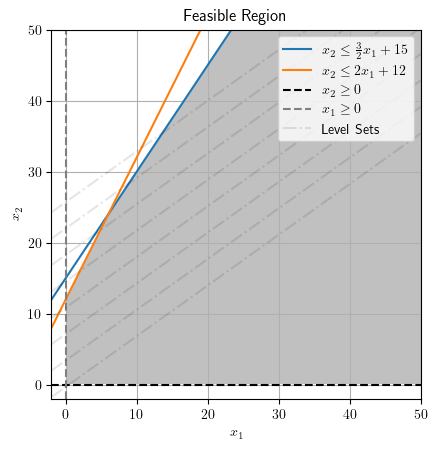
\includegraphics[width=0.6\textwidth]{problem_5i.png}
    \caption{Feasible Region for minimizing $z = -5x_1 - 7x_2$}
    \label{fig:problem_5i}
  \end{figure}
  \ \\
\end{solution}
  \pagebreak
  \item Show that the second-order sufficiency conditions do not hold anywhere, but that any point $x_*$ which satisfies the
first-order necessary conditions is a global minimizer.

\textit{Hint: } Show that there are no feasible directions of descent at $x_*$, and that this implies that $x_*$ is a
global minimizer.

\begin{solution}
    \ \\
    \vfill
\end{solution}
  \pagebreak
  \item Determine two linearly independent directions of unboundedness.

\begin{solution}
  \ \\
  \vfill
  \ \\
\end{solution}
\end{enumerate}
